\subsection{Class diagrams}

Các class diagram được nhóm thiết kế theo mô hình kiến trúc MVC (Model-Controller-View). Mỗi tầng đảm nhiệm mỗi nhóm chức năng trong hệ thống:
\begin{itemize}
    \item Tầng View: lắng nghe sự kiện, thu nhận dữ liệu và tương tác người dùng để chuyển đến Controller xử lý; hiển thị dữ liệu do Controller chuyển giao từ Model lên, hiển thị các
giao diện, biểu mẫu xác nhận, thông báo, nhập liệu.
    \item Tầng Controller: xử lý sự kiện, điều khiển luồng dữ liệu, cập nhật giao diện.
    \item Tầng Model: lưu trữ dữ liệu hệ thống và cung cấp phương thức cơ bản xử lý logic nghiệp
vụ.
\end{itemize}
\subsubsection{Xác thực}
\begin{figure}[H]
    \begin{center}
        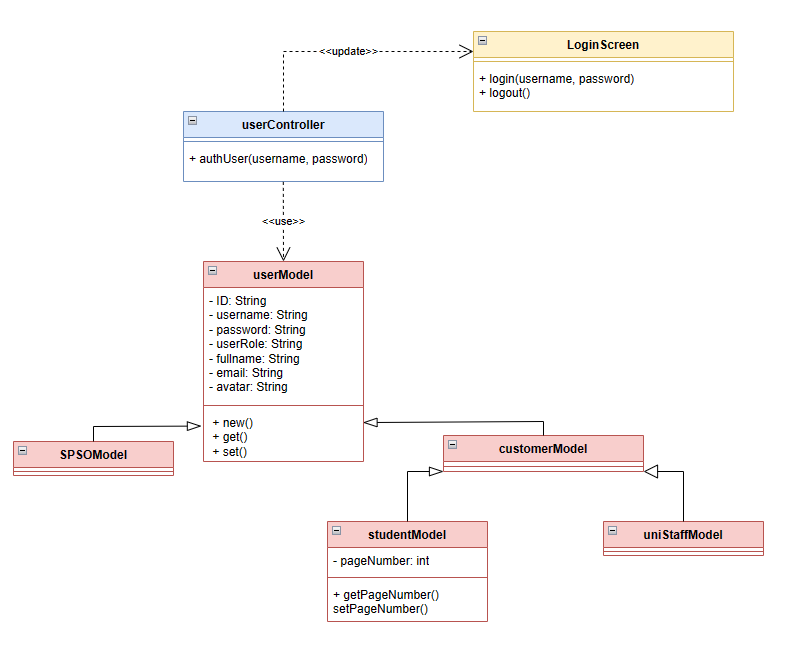
\includegraphics[width=0.9\textwidth]{Images/System Modelling/Authen_Class.png}
        \caption{Class diagram cho module xác thực tài khoản}
    \end{center}
\end{figure}

\subsubsection{In}
\begin{figure}[H]
    \begin{center}
        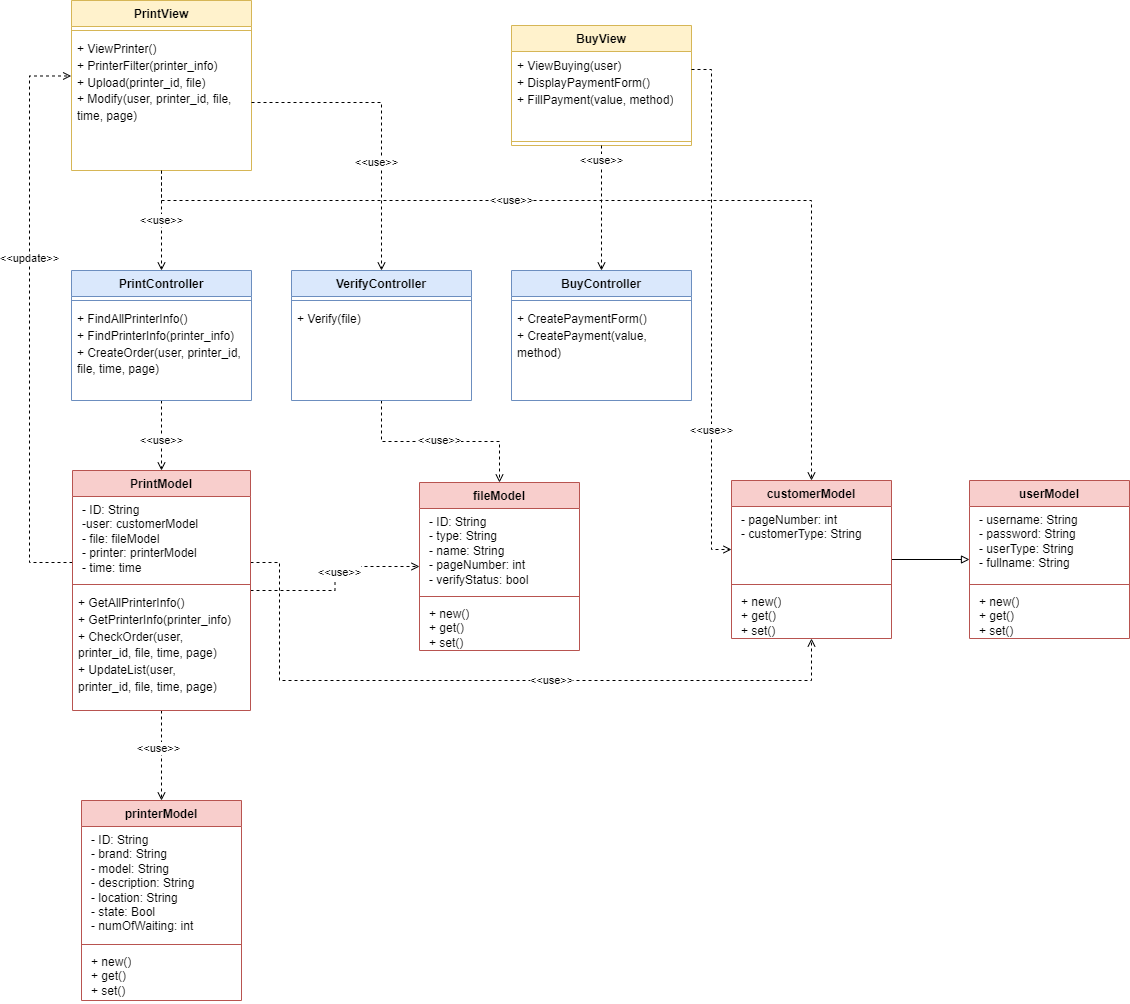
\includegraphics[width=0.9\textwidth]{Images/System Modelling/Printing_Class.png}
        \caption{Class diagram cho module in}
    \end{center}
\end{figure}

\subsubsection{Quản lý máy in}
\begin{figure}[H]
    \begin{center}
        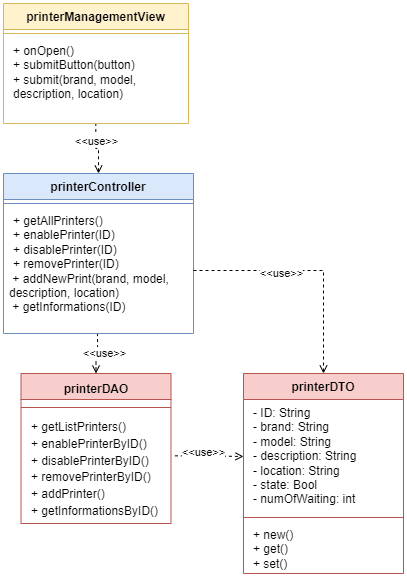
\includegraphics[width=0.7\textwidth]{Images/System Modelling/PM_Class.png}
        \caption{Class diagram cho module quản lý máy in}
        \label{fig:arch}
    \end{center}
\end{figure}
\subsubsection{Quản lý in ấn (bao gồm định dạng tệp cho phép in và quản lí tặng giấy)}
\begin{figure}[H]
    \begin{center}
        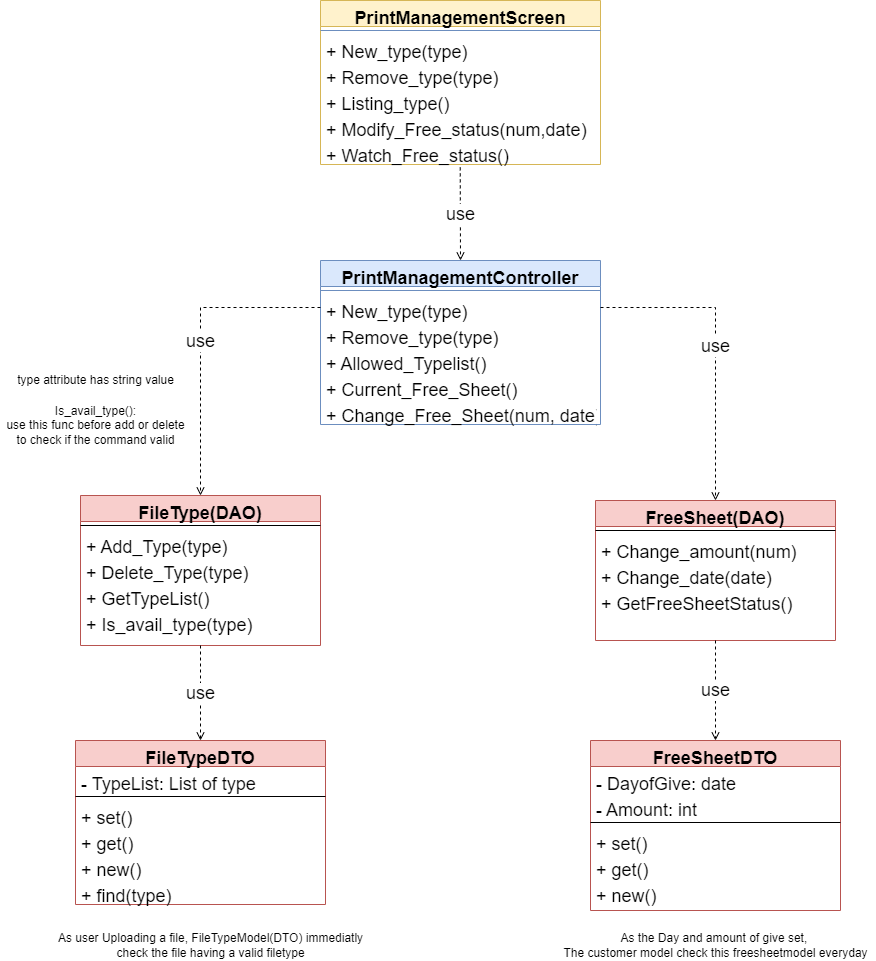
\includegraphics[width=0.9\textwidth]{Images/System Modelling/PS_Class.png}
        \caption{Class diagram cho module quản lý in ấn (bao gồm định dạng tệp cho phép in và quản lí tặng giấy)}
        \label{fig:arch}
    \end{center}
\end{figure}
\subsubsection{Lịch sử in}
\begin{figure}[H]
    \begin{center}
        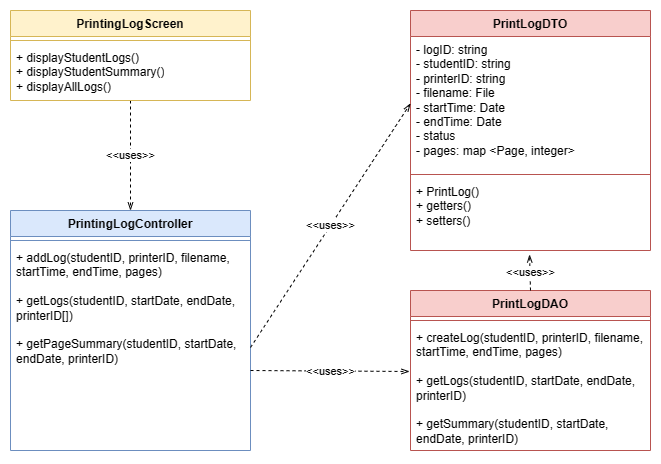
\includegraphics[width=0.9\textwidth]{Images/System Modelling/Logging_Class.png}
        \caption{Class diagram cho module lịch sử in}
        \label{fig:arch}
    \end{center}
\end{figure}